\documentclass[aspectratio=169]{beamer}

\usepackage[utf8]{inputenc}
\usepackage{amsmath, amssymb}
\usepackage{graphicx}
\usepackage{booktabs}
\usepackage{hyperref}
\usepackage{xcolor}
\usepackage{tikz}
\usetikzlibrary{positioning, arrows.meta, calc}

% --- Theme (simple, close to your existing deck style) ---
\usetheme{Madrid}
\usecolortheme{default}

\definecolor{cnamred}{RGB}{179,0,26}
\definecolor{orange}{RGB}{255, 140, 0}

\setbeamercolor{frametitle}{bg=cnamred, fg=white}
\setbeamercolor{structure}{fg=cnamred}
\setbeamercolor{palette primary}{bg=cnamred, fg=white}
\setbeamertemplate{navigation symbols}{}

\setbeamercolor{palette secondary}{bg=cnamred!90, fg=white}
\setbeamercolor{palette tertiary}{bg=cnamred!80, fg=white}
\newcommand{\hl}[1]{\textcolor{cnamred}{\textbf{#1}}}
\newcommand{\warn}[1]{\textcolor{orange}{\textbf{#1}}}


\setbeamertemplate{headline}{%
  \begin{beamercolorbox}[wd=\paperwidth,ht=3.2ex,dp=1.2ex,leftskip=0.3cm,rightskip=0.3cm]{frametitle}%
    \hfill\raisebox{-1ex}{\includegraphics[height=6mm]{cnam-logo.png}}\hspace{0.15cm}%
  \end{beamercolorbox}%
}

\setbeamertemplate{footline}{%
\hfill\begin{beamercolorbox}[sep=2pt,ht=2.5ex,dp=1ex]{footline}%
\usebeamerfont{footline}\insertframenumber{} / \inserttotalframenumber\hspace{0.5cm}%
\end{beamercolorbox}%
}
\setbeamertemplate{navigation symbols}{}

% --- Title info ---
\title{ATLAS: Adaptive Task-aware Federated Learning for LLMs}
\subtitle{Advanced Master's Project}

\author{Mahmoud Mayaleh \\[6pt] \small Prof. Lyes Khoukhi (CNAM, France) \and Zakaria Abou El Houda (INRS, Canada)}

\date{February 23, 2026}

\begin{document}

% =========================================================
% 1) TITLE
% =========================================================
\begin{frame}
  \titlepage
\end{frame}

% =========================================================
% 2) PROJECT SUBJECT (1 slide)
% =========================================================
\begin{frame}{Project Subject}
\textbf{Context:} Fine-tuning Large Language Models (LLMs) on distributed users/devices without collecting data centrally.

\vspace{0.3cm}
\textbf{Problem:} Federated Learning for LLMs faces:
\begin{itemize}
  \item \hl{Privacy constraints}: data stays on-device.
  \item \hl{Heterogeneity}: clients have different tasks + different resources (CPU/low RAM vs GPU).
  \item \hl{Cost}: communication and memory make full fine-tuning impractical.
\end{itemize}

\vspace{0.3cm}
\textbf{Objective:} Design and implement \hl{ATLAS}, a practical pipeline that:
\begin{itemize}
  \item learns across multiple tasks without harmful mixing,
  \item adapts to device constraints,
  \item keeps communication manageable,
  \item preserves personalization.
\end{itemize}
\end{frame}

% =========================================================
% 3-4) TECHNOLOGICAL CONTEXT (1-2 slides)
% =========================================================
\begin{frame}{Technological Context (1/2): Federated Learning + LLMs}
\textbf{Federated Learning (FL):}
\begin{itemize}
  \item Clients train locally and share updates (not raw data).
  \item Server aggregates information across clients/rounds.
\end{itemize}

\vspace{0.3cm}
\textbf{Why LLMs make FL harder:}
\begin{itemize}
  \item Model size $\rightarrow$ \warn{memory and compute pressure} on edge devices.
  \item Sharing large updates $\rightarrow$ \warn{high communication cost}.
  \item Multi-task reality $\rightarrow$ \warn{negative transfer} if everything is averaged globally.
\end{itemize}

\vspace{0.3cm}
\textbf{Key idea:} Make FL for LLMs feasible via \hl{task awareness} + \hl{parameter efficiency}.
\end{frame}

\begin{frame}{Technological Context (2/2): PEFT (LoRA) + Split Learning}
\textbf{Parameter-Efficient Fine-Tuning (PEFT): LoRA}
\begin{itemize}
  \item Train small low-rank adapters instead of all parameters.
  \item Reduces trainable parameters and memory footprint.
\end{itemize}

\vspace{0.3cm}
\textbf{Split Learning (client/server split):}
\begin{itemize}
  \item Client runs early layers, server runs later layers.
  \item Exchange activations/gradients instead of full model states.
  \item Enables training with \hl{very limited client memory}.
\end{itemize}

\vspace{0.3cm}
\textbf{ATLAS uses both:} LoRA for efficiency + split FL for device feasibility.
\end{frame}

% =========================================================
% 5) BASE SPECIFICATIONS (1 slide)
% =========================================================
\begin{frame}{Base Specifications (Scope + Constraints)}
\textbf{Scope (pipeline):}
\begin{itemize}
  \item Multi-task FL setting (clients partitioned across tasks).
  \item Transformer backbone(s) (e.g., DistilBERT/BERT/RoBERTa/GPT-2).
\end{itemize}

\vspace{0.2cm}
\textbf{Tasks / datasets (example configuration):}
\begin{itemize}
  \item NLP classification tasks (e.g., SST-2, MRPC, CoLA, QNLI).
\end{itemize}

\vspace{0.2cm}
\textbf{Operational constraints:}
\begin{itemize}
  \item Heterogeneous client memory budgets and compute.
  \item Practical runtime limits (session-based / checkpoint resume).
\end{itemize}

\vspace{0.2cm}
\textbf{Evaluation targets:}
\begin{itemize}
  \item Accuracy/F1 (per task and average), stability (variance), and communication (MB).
\end{itemize}
\end{frame}

% =========================================================
% 6-8) ANALYSIS (2-3 slides)
% =========================================================
\begin{frame}{Analysis (1/2): What Must Be Solved}
\textbf{Main challenges identified:}
\begin{enumerate}
  \item \hl{Task heterogeneity}: different tasks should not be blindly averaged.
  \item \hl{Resource heterogeneity}: ranks/splits must adapt to each client.
  \item \hl{Communication}: must stay low enough to be realistic.
  \item \hl{Personalization}: improve per-client performance, not just global average.
\end{enumerate}

\vspace{0.3cm}
\textbf{Design requirement:} An end-to-end method that is implementable, reproducible, and supports ablations/baselines.
\end{frame}

\begin{frame}{Analysis (2/2): ATLAS Pipeline (4 Phases)}
\textbf{ATLAS is a structured 4-phase pipeline:}
\begin{enumerate}
  \item \hl{Phase 1: Task clustering} via privacy-preserving fingerprints.
  \item \hl{Phase 2: Heterogeneous LoRA configuration} (rank allocation under budgets).
  \item \hl{Phase 3: Split federated learning} with task-aware aggregation + adaptive split selection.
  \item \hl{Phase 4: Laplacian regularization} for graph-based personalization.
\end{enumerate}

\vspace{0.3cm}
\begin{center}
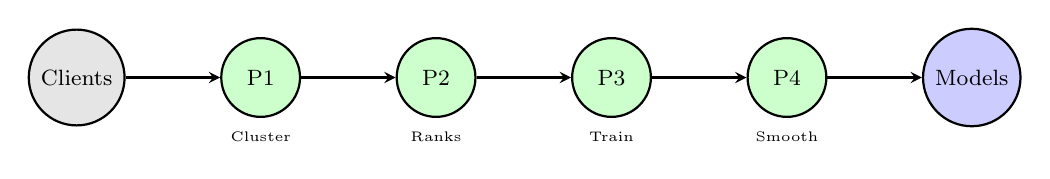
\begin{tikzpicture}[node distance=1.2cm, every node/.style={font=\footnotesize}]

% Icons (use shapes)
\node[circle, draw, thick, fill=gray!20, minimum size=1cm] (c) {Clients};
\node[circle, draw, thick, fill=green!20, minimum size=1cm, right=of c] (p1) {P1};
\node[circle, draw, thick, fill=green!20, minimum size=1cm, right=of p1] (p2) {P2};
\node[circle, draw, thick, fill=green!20, minimum size=1cm, right=of p2] (p3) {P3};
\node[circle, draw, thick, fill=green!20, minimum size=1cm, right=of p3] (p4) {P4};
\node[circle, draw, thick, fill=blue!20, minimum size=1cm, right=of p4] (o) {Models};

% Arrows
\foreach \from/\to in {c/p1, p1/p2, p2/p3, p3/p4, p4/o}
  \draw[->, >=stealth, thick] (\from) -- (\to);

% Labels
\node[below=0.05cm of p1] {\tiny Cluster};
\node[below=0.05cm of p2] {\tiny Ranks};
\node[below=0.05cm of p3] {\tiny Train};
\node[below=0.05cm of p4] {\tiny Smooth};

\end{tikzpicture}
\end{center}
\end{frame}


\begin{frame}{System Diagram}
\begin{center}
    
\includegraphics[width=0.65\linewidth]{figures/atlas-diagram.png}
\end{center}
\end{frame}

% =========================================================
% 9-12) DEVELOPMENTS ACHIEVED (4-7 slides)
% =========================================================
\begin{frame}{Developments Achieved (1/4): Phase 1 --- Task Clustering}
\textbf{What was implemented:}
\begin{itemize}
  \item Privacy-preserving fingerprint extraction (captures task signal without raw data).
  \item Similarity-based clustering to group clients by task.
  \item Cluster alignment across rounds (stable IDs for consistent aggregation).
\end{itemize}

\vspace{0.3cm}
\textbf{How it works:}
\begin{enumerate}
  \item Each client computes gradient-based fingerprint on local data.
  \item Server clusters fingerprints (e.g., K-means on embeddings).
  \item Match clusters across rounds to prevent label flipping.
\end{enumerate}

\end{frame}


\begin{frame}{Developments Achieved (2/4): Phase 2 --- HSplitLoRA (Heterogeneous Ranks)}
\textbf{What was implemented:}
\begin{itemize}
  \item Per-client LoRA rank allocation based on memory/compute budgets.
  \item Automatic rank selection (low-rank for weak devices, higher for strong devices).
  \item Optional: Adjust for cluster/task complexity.
\end{itemize}

\vspace{0.3cm}
\textbf{How it works:}
\begin{columns}[T]
\column{0.48\textwidth}
\textbf{Weak client (4GB RAM):}
\begin{itemize}
  \item Rank $r=4$ (first layers only)
  \item $\approx 0.1$M trainable params
  \item Fits low-end devices
\end{itemize}

\column{0.48\textwidth}
\textbf{Strong client (16GB RAM):}
\begin{itemize}
  \item Rank $r=16$ (all attention layers)
  \item $\approx 0.5$M trainable params
  \item Full expressivity
\end{itemize}
\end{columns}

\vspace{0.3cm}
\textbf{Difficulty encountered:} Fixed ranks fail on low-memory devices.

\textbf{Outcome:} \textcolor{green}{\textbf{Supports 4GB–32GB clients}} with optimal performance.
\end{frame}


\begin{frame}{Developments Achieved (3/4): Phase 3 --- Split FL + Adaptive Split Selection}
\textbf{What was implemented:}
\begin{itemize}
  \item Split learning workflow (client prefix / server suffix).
  \item Task-aware aggregation inside clusters.
  \item Adaptive split selection using a weighted objective.
\end{itemize}

\vspace{0.3cm}
\textbf{How split selection works:}
\begin{itemize}
  \item \textbf{Memory cost}: Fit client's available RAM (higher layers $\rightarrow$ more memory).
  \item \textbf{Communication}: Minimize activation/gradient transfer size.
  \item \textbf{Importance}: Prioritize layers critical for task accuracy.
  \item \textbf{Balance}: Distribute workload fairly across client-server.
\end{itemize}

\end{frame}


\begin{frame}{Developments Achieved (4/4): Phase 4 --- Laplacian Personalization}
\textbf{What was implemented:}
\begin{itemize}
  \item Similarity graph between clients (from fingerprints).
  \item Laplacian regularization to encourage smoothness within neighborhoods.
  \item Clients with similar tasks share knowledge via graph-based weighting.
\end{itemize}

\vspace{0.3cm}
\textbf{How it works:}
\begin{itemize}
  \item \textbf{Step 1:} Compute pairwise similarity between client fingerprints.
  \item \textbf{Step 2:} Build adjacency graph (closer fingerprints $\rightarrow$ stronger connections).
  \item \textbf{Step 3:} Regularize model updates to be smooth across connected clients.
\end{itemize}

\end{frame}


% =========================================================
% 13) RESULTS
% =========================================================

\begin{frame}{Experimental Setup}
\textbf{Baselines:}
\begin{itemize}
  \item \hl{Standard FL}: global FedAvg across all clients (no clustering).
  \item \hl{FedAvg (Clustered)}: task-aware FedAvg after client clustering (no hetero-LoRA / no split / no Laplacian).
  \item \hl{ATLAS - No Laplacian}: full ATLAS pipeline except Laplacian regularization (ablation).
  \item \hl{ATLAS (Full)}: Phases 1--4 (clustering, heterogeneous LoRA allocation, split FL, Laplacian personalization).
\end{itemize}

\vspace{0.1cm}
\textbf{Protocol:}
\begin{itemize}
  \item Training rounds: $\mathbf{10}$ rounds.
  \item Local epochs: $\mathbf{3}$ per round.
  \item Models evaluated: DistilBERT, GPT-2, and Qwen2.5-0.5B.
  \item Tasks/datasets: GLUE subset (SST-2, MRPC, CoLA, QNLI).
  \item Device mixes: heterogeneous client profiles (smartphone/tablet / laptop\_cpu / laptop\_gpu)
  \item Random seeds: 42, 123, 456 (reported mean $\pm$ std across seeds).
\end{itemize}

\end{frame}

\begin{frame}{Results (1/3): Baselines + Task Clustering Visualization}
\begin{columns}[T]
\column{0.62\textwidth}
\textbf{Cross-model baseline comparison (3 seeds):}
\begin{center}
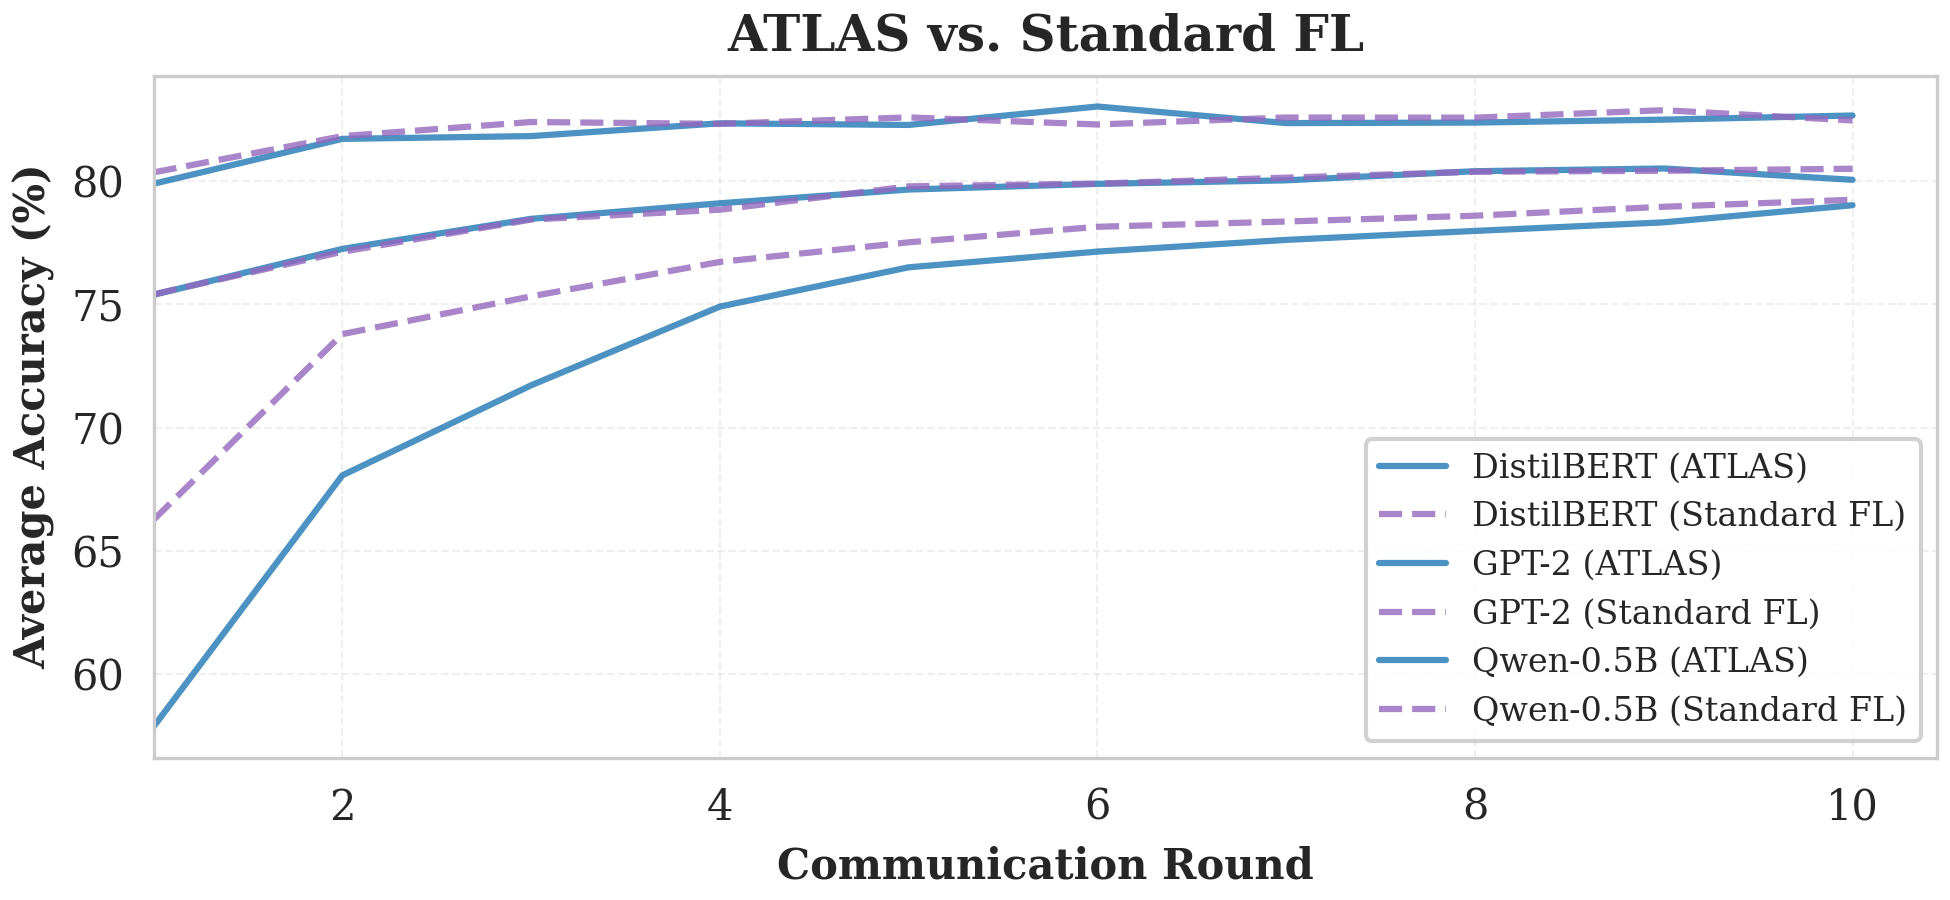
\includegraphics[width=\linewidth]{figures/fig2_model_baseline.png}
\end{center}

\column{0.38\textwidth}
\textbf{Fingerprint map (clients cluster by task):}
\begin{center}

\includegraphics[width=\linewidth]{figures/fig9_fingerprint_map.png}
\end{center}
\end{columns}

\vspace{0.15cm}
\scriptsize
\textbf{Experiment breadth:} DistilBERT, GPT-2, Qwen2.5-0.5B; multiple FL baselines (Standard FL, FedAvg-Clustered) vs ATLAS; mean across seeds (42/123/456).
\end{frame}

\begin{frame}{Results (2/3): Communication Efficiency (ATLAS $>$ FedAvg $>$ Standard FL)}
\begin{columns}[T]
\column{0.57\textwidth}
\begin{center}

\includegraphics[width=0.9\linewidth]{figures/fig3_accuracy_vs_communication.png}
\end{center}

\column{0.43\textwidth}
\textbf{DistilBERT (LoRA): Comm. to Reach Thresholds}

\vspace{0.1cm}
\scriptsize
\begin{tabular}{lrr}
\toprule
Method & Threshold & Comm. (MB)\\
\midrule
ATLAS & 75\% (r=1) & 69.4 \\
ATLAS & 77\% (r=2) & 138.8 \\
ATLAS & 80\% (r=5) & 347.0 \\
\midrule
FedAvg (Clust.) & 75\% (r=1) & 94.7 \\
FedAvg (Clust.) & 77\% (r=2) & 189.4 \\
FedAvg (Clust.) & 80\% (r=6) & 568.3 \\
\midrule
Standard FL & 75\% (r=2) & 149.0 \\
Standard FL & 77\% (r=3) & 223.4 \\
Standard FL & 80\% (r=7) & 521.2 \\
\bottomrule
\end{tabular}
\scriptsize

\textbf{Takeaway:} ATLAS reaches each accuracy threshold with substantially less communication than baselines, 75\%: ATLAS 69.4 MB → full fine-tuning \textasciitilde 31,941\,MB (\textasciitilde 31.9\,GB).

\end{columns}
\end{frame}

\begin{frame}{Results (3/3): Parameter Efficiency + Heterogeneous LoRA Allocation}
\begin{columns}[T]
\column{0.48\textwidth}
\textbf{ATLAS vs full fine-tuning (Qwen2.5-0.5B):}
\begin{center}

\includegraphics[width=\linewidth]{figures/fig_atlas_vs_qwen_params.png}
\end{center}

\column{0.52\textwidth}
\textbf{Per-device trainable parameters (heterogeneous ranks):}
\begin{center}

\includegraphics[width=\linewidth]{figures/fig_device_allocation.png}
\end{center}
\end{columns}
\end{frame}

% =========================================================
% 14) SUMMARY (1 slide)
% =========================================================
\begin{frame}{Summary: ATLAS Key Contributions}

\textbf{What ATLAS delivers:}

\vspace{0.5cm}

\begin{itemize}
  \item \hl{Task-aware learning}: Clustering reduces negative transfer across heterogeneous tasks.
  
  \item \hl{Device-aware training}: Heterogeneous LoRA ranks + adaptive split points accommodate diverse resource constraints.
 \item \hl{Scalable communication}: 
\textbf{65\% reduction vs. FedAvg-LoRA} \& \textbf{99.8\% reduction vs. full FT} 
  \item \hl{Personalization}: Laplacian regularization improves client-level consistency and reduces variance.
\end{itemize}

\vspace{0.5cm}

\begin{block}{Bottom Line}
\centering
\textbf{ATLAS makes federated LLM fine-tuning practical:} \\
Train 0.5\% parameters · 20$\times$ less communication · Preserve task performance
\end{block}

\end{frame}


\end{document}